% Appendix C-E - Apendices de Desarrollo

%\chapter{Frequently Asked Questions} % Main appendix title

\chapter{Preparaciones de Desarrollo}
\label{AnexoC} % For referencing this appendix elsewhere, use \ref{AppendixA}

\section{Servicios Nativos}
% TODO: Intro to Section?

\subsection{Servidor de Git}
Instalar paquetes para un interfaz web sencilla de Git:
\begin{lstlisting}
apt install git gitweb fcgiwrap
\end{lstlisting}

Se crea un usuario del sistema operativo solo para Git:
\begin{lstlisting}
adduser git
\end{lstlisting}

Se autentica como el usuario creado:
\begin{lstlisting}
su - git
\end{lstlisting}

Para tener repositorios ejemplares, se clona algunos repositorios:
\begin{lstlisting}
git clone --bare\
	https://gitlab.com/nishedcob/GitEDU.git\
	repositories/GitEDU.git
git clone --bare\
	https://gitlab.com/ArqAppGrpBravoEarleyVargas/\
    	GitEduERP.git\
	repositories/GitEduERP.git
\end{lstlisting}

Entrar al directorio de repositorios y arreglar permisos para permitir git push desde repositorios remotos:
\begin{lstlisting}
cd repositories/
for repo in `ls`; do
	cd $repo;
    pwd;
    chmod -R g+ws .;
    chgrp -R git .;
    git --bare update-server-info;
    cp hooks/post-update.sample hooks/post-update;
    chmod a+x hooks/post-update;
    cd ..;
done
\end{lstlisting}

Después se configura NGinX para trabajar con gitweb:
\begin{lstlisting}
# NGinX Config:
server {
        listen 80;
        listen [::]:80;
        server_name git.localhost 192.168.99.1 10.10.10.1;
        root /usr/share/gitweb;
        access_log /var/log/nginx/gitweb.access.log;
        # static repo files for cloning over https
        location ~ ^.*\.git/objects/([0-9a-f]+/[0-9a-f]+\
        	|pack/pack-[0-9a-f]+.(pack|idx))$ {
                root /home/git/repositories/;
        }

        # requests that need to go to git-http-backend
        location ~ ^.*\.git/(HEAD|info/refs|objects/info/.*\
        	|git-(upload|receive)-pack)$ {
                root /home/git/repositories;

                fastcgi_pass unix:/var/run/fcgiwrap.socket;
                fastcgi_param SCRIPT_FILENAME   /usr/lib/\
                	git-core/git-http-backend;
                fastcgi_param PATH_INFO          $uri;
                fastcgi_param GIT_PROJECT_ROOT  /home/git/\
                	repositories;
                fastcgi_param GIT_HTTP_EXPORT_ALL "";
                fastcgi_param REMOTE_USER $remote_user;
                include fastcgi_params;
        }

        # send anything else to gitweb if it's not a real file
        try_files $uri @gitweb;
        location @gitweb {
                fastcgi_pass unix:/var/run/fcgiwrap.socket;
                fastcgi_param SCRIPT_FILENAME   /usr/share/\
                	gitweb/gitweb.cgi;
                fastcgi_param PATH_INFO          $uri;
                fastcgi_param GITWEB_CONFIG      /etc/gitweb\
                	.conf;
                include fastcgi_params;
        }
}
\end{lstlisting}

Además se configura gitweb con la siguiente configuración:
\begin{lstlisting}
# Edit /etc/gitweb.conf
# path to git projects (<project>.git)
#$projectroot = "/var/lib/git";
$projectroot = "/home/git/repositories";
\end{lstlisting}

Prueba de que funciona:
\begin{lstlisting}
git clone http://git.localhost/nishedcob/GitEDU.git \
	GitEDU-test
\end{lstlisting}

Dado que el mismo GitWeb no tenga problemas con bajada de datos (\texttt{git fetch} / \texttt{git pull} / \texttt{git clone}) pero si tiene problemas con subida de datos como se lo require en EduNube para armar repositorios de ejecuccion validadas, se ve una necesidad de habilitar subida al mismo por SSH:

Como root en el servidor de Git, se cambia la clave del usuario de Git:
\begin{lstlisting}
passwd git
\end{lstlisting}

Como el usuario de EduNube en el servidor para el mismo:
\begin{lstlisting}
cd .ssh/
# Deja la llave generada sin clave:
ssh-keygen -f id_git
# Copia la llave publica al servidor
ssh-copy-id -i ~/.ssh/id_git.pub git@10.10.10.1
# Prueba que funciona
ssh -i ~/.ssh/id_git -vvv git@10.10.10.1
# Guardar la configuracion:
cat >> ~/.ssh/config < EOF

Host git
     HostName 10.10.10.1
     User git
     Port 22
     IdentityFile $HOME/.ssh/id_git

EOF
# Probar con:
ssh -vvv git
\end{lstlisting}

\section{Servicios Virtualizados}
% TODO: Section Introduction?

\subsection{Maquina Virtual de Xen para Moodle}
Para el ambiente de Moodle (LMS \index{LMS} contra el cual se ha llevado el desarrollo), se crea una maquina virtual de Debian Stretch (9) con 1 GiB de RAM, 1 CPU virtual, 6 GiB de disco, 512 MiB de intercambio y una dirección IP fija de 10.10.10.10. Los resultados del mismo comando se puede ver en la figura \ref{vm-moodle}.
\begin{lstlisting}
	xen-create-image --hostname=debian-moodle\
    		--ip=10.10.10.10 --netmask=255.255.255.0\
        	--gateway=10.10.10.1 --memory=1024mb\
        	--vcpus=1 --lvm=Xephyr-VG --pygrub\
        	--dist=stretch --force --size=6144mb\
        	--swap=512mb
\end{lstlisting}

\begin{figure}
	\begin{center}
    	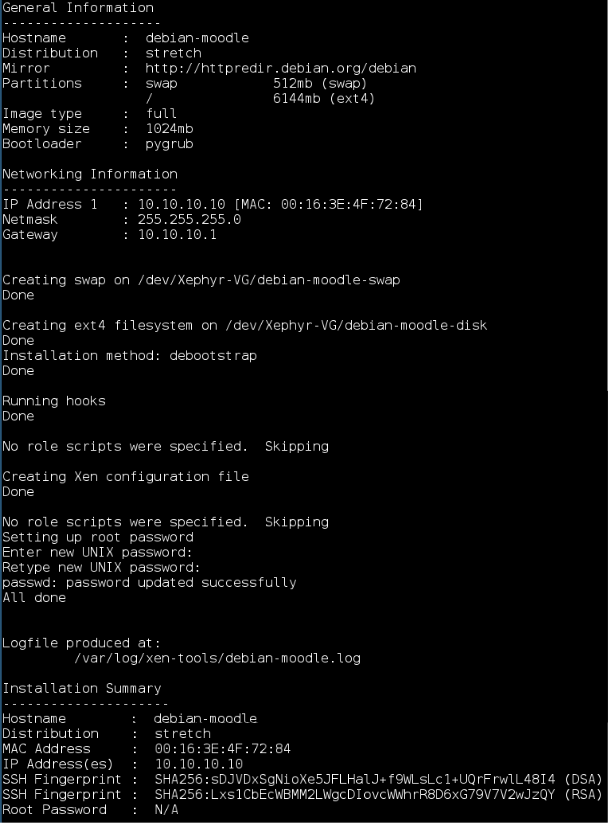
\includegraphics[width=0.75\textwidth]{Figures/crear-moodle.png}
    \end{center}
  	\caption{Crear maquina virtual para Moodle.}
    \label{vm-moodle}
\end{figure}

Se renombró el archivo de configuración de la maquina virtual generado en el paso anterior para temas de consistencia.

\begin{lstlisting}
	mv /etc/xen/debian-moodle.cfg\
    		/etc/xen/domU-debian-moodle.cfg
\end{lstlisting}

Un bug de Xen-Tools causa que no se instala correctamente un núcleo de Linux en la maquina virtual y por lo tanto es necesario entrar al mismo con un Chroot y instalar los paquetes faltantes (y hacer las adecuadas configuraciones para permitir su arranque independiente de ayuda externa)\footnote{6 meses despues de la redaccion de estos pasos, y Xen-Tools ya no tiene este bug, motivo por el cual se puede emitir este paso si es que la maquina virtual esta funcionando de forma correcta.}.

\begin{lstlisting}
	mount /dev/Xephyr-VG/debian-moodle-disk /mnt
	mount -o bind /proc /mnt/proc
	mount -o bind /sys /mnt/sys
	mount -o bind /dev /mnt/dev
	cp /etc/resolv.conf /mnt/etc/resolv.conf
	chroot /mnt /bin/bash
	apt install linux-image-amd64
	vim.tiny /boot/grub/menu.lst
	# Revisar que los archivos referenciados existen
	#		de verdad por ejemplo:
	# Replace initrd.img- con initrd.img
    # guarda y sale
	exit
	umount /mnt/proc            
	umount /mnt/sys 
	umount /mnt/dev 
	umount /mnt	
\end{lstlisting}

Para levantar la maquina virtual:

\begin{lstlisting}
	xl create /etc/xen/domU-debian-moodle.cfg -c
\end{lstlisting}

Se debe seleccionar la tercera opción (Default Kernel).

Se puede dar una revisión a la configuración de red para asegurarse de que esta correcto:

\begin{lstlisting}
	vim.tiny /etc/network/interfaces
\end{lstlisting}

Debe contener:

\begin{lstlisting}
auto eth0
iface eth0 inet static
 address 10.10.10.10
 gateway 10.10.10.1
 netmask 255.255.255.0
\end{lstlisting}

En el presente caso, Xen-Tools logró configurar esta parte de forma correcta.

A continuación se procede con la instalación de Moodle:

\begin{lstlisting}
# actualiza el sistema
apt update
apt upgrade

# instala dependencias
apt install apache2 php7.0 mysql-server php7.0-mysql
apt install libapache2-mod-php7.0 php7.0-gd php7.0-curl
apt install php-xml php-zip php-mbstring php-soap
apt install php7.0-xmlrpc php7.0-intl
vim.tiny /etc/php/7.0/apache2/php.ini

# agrega:
extension=mysql.so 
extension=gd.so

# edita:

memory_limit = 40M
# dejado con el valor por defecto de 128M

post_max_size = 80M
upload_max_filesize = 80M

# guarda y sale

# reinicia apache para coger los cambios
systemctl restart apache2

\end{lstlisting}

A continuación se configura la base de datos:

\begin{lstlisting}

# clave de root es root
mysqladmin -u root password "root"

# iniciar session como root
mysql -u root -p

# crear base de datos y hacer que ocupa UTF-8
mysql> CREATE DATABASE moodle;
mysql> ALTER DATABASE moodle charset=utf8;
mysql> exit;

## No se implemento ##
# Moodle queja de UTF8

# Se podria arreglar
# (antes de instalar Moodle)
# con:

mysql -u root -p

mysql> ALTER DATABASE moodle charset=utf8mb4;
mysql> exit;
######################

systemctl restart mysql

\end{lstlisting}

Se realiza la instalación de la ultima versión de Moodle (3.3 con sus respectivos patches de fallas desde que el mismo salio):

\begin{lstlisting}

# descargar
wget https://download.moodle.org/download.php/direct/stable33/\
	moodle-latest-33.tgz

# descomprimir
tar -zxvf moodle-latest-33.tgz

# meter en la ubicacion para apache
mv moodle /var/www

# ir a ubicacion para apache
cd /var/www

# crear ubicacion para datos
mkdir moodledata

# arreglar permisos
chown -R www-data:www-data moodle
chown -R www-data:www-data moodledata
chmod -R 755 moodle
chmod -R 755 moodledata

# modificar configuracion de apache
vim.tiny /etc/apache2/sites-available/000-default.conf

# editar
DocumentRoot "/var/www/moodle"

# guardar y salir

# reiniciar apache para aplicar los cambios
systemctl restart apache2

\end{lstlisting}

Arreglar la base de datos para que acepte conexiones desde Moodle:

\begin{lstlisting}

mysql -u root -p

GRANT ALL PRIVILEGES on *.* to
	'root'@'localhost' IDENTIFIED BY 'root';
GRANT ALL PRIVILEGES on *.* to
	'root'@'localhost' IDENTIFIED BY 'root';
FLUSH PRIVILEGES;
exit;

\end{lstlisting}

Para seguir con la instalación se abre un navegador con la dirección \url{http://10.10.10.10/} para seguir las instrucciones que se le lleve por toda la configuración inicial del Moodle.

Al final se agregue un trabajo de cron para ayudar con los tareas periódicas que Moodle requiere para su mantenimiento continuo:

\begin{lstlisting}

crontab -u www-data -e
# add line:
*/10 * * * * /usr/bin/php
		/var/www/moodle/admin/cli/cron.php
        		>/dev/null

\end{lstlisting}

Estos pasos fueron adaptados de la guía oficial del proyecto de Moodle para instalación en Debian \citep{MOODLE-Install-Debian}.

Ahora que todo esta funcionando se recomienda editar /boot/grub/menu.lst para comentar las entradas del pyGrub que son defectuosas (los primeros dos) para que se puede levantar la maquina virtual sin intervención humana.

\subsection{Máquina Virtual de Xen}
Para crear el servidor de Git con GitLab Community Edition, se va a empezar con las mismas piezas del servidor del LMS/Moodle, es decir una maquina virtual de Debian 9. El mismo se crea como una maquina virtual de Debian Stretch (9) con 1 GiB de RAM, 1 CPU virtual, 6 GiB de disco, 512 MiB de intercambio y una dirección IP fija de 10.10.10.11.
\begin{lstlisting}
	xen-create-image --hostname=debian-gitlab\
    		--ip=10.10.10.11 --netmask=255.255.255.0\
        	--gateway=10.10.10.1 --memory=1024mb\
        	--vcpus=1 --lvm=Xephyr-VG --pygrub\
        	--dist=stretch --force --size=6144mb\
        	--swap=512mb
\end{lstlisting}

Se renombró el archivo de configuración de la maquina virtual generado en el paso anterior para temas de consistencia.

\begin{lstlisting}
	mv /etc/xen/debian-gitlab.cfg\
    		/etc/xen/domU-debian-gitlab.cfg
\end{lstlisting}

Un bug de Xen-Tools causa que no se instala correctamente un núcleo de Linux en la maquina virtual y por lo tanto es necesario entrar al mismo con un Chroot y instalar los paquetes faltantes (y hacer las adecuadas configuraciones  para permitir su arranque independiente de ayuda externa)\footnote{6 meses despues de la redaccion de estos pasos, y Xen-Tools ya no tiene este bug, motivo por el cual se puede emitir este paso si es que la maquina virtual esta funcionando de forma correcta.}.

\begin{lstlisting}
	mount /dev/Xephyr-VG/debian-gitlab-disk /mnt
	mount -o bind /proc /mnt/proc
	mount -o bind /sys /mnt/sys
	mount -o bind /dev /mnt/dev
	cp /etc/resolv.conf /mnt/etc/resolv.conf
	chroot /mnt /bin/bash
	apt install linux-image-amd64
	vim.tiny /boot/grub/menu.lst
	# Revisar que los archivos referenciados existen
	#		de verdad por ejemplo:
	# Replace initrd.img- con initrd.img
    # guarda y sale
	exit
	umount /mnt/proc            
	umount /mnt/sys 
	umount /mnt/dev 
	umount /mnt	
\end{lstlisting}

Para levantar la maquina virtual:

\begin{lstlisting}
	xl create /etc/xen/domU-debian-gitlab.cfg -c
\end{lstlisting}

Se debe seleccionar la tercera opción (Default Kernel).

Se puede dar una revisión a la configuración de red para asegurarse de que esta correcto:

\begin{lstlisting}
	vim.tiny /etc/network/interfaces
\end{lstlisting}

Debe contener:

\begin{lstlisting}
auto eth0
iface eth0 inet static
 address 10.10.10.11
 gateway 10.10.10.1
 netmask 255.255.255.0
\end{lstlisting}

En el presente caso, Xen-Tools logró configurar esta parte de forma correcta.

A continuación se procede con la instalación de Gitlab:

\begin{lstlisting}
# actualiza el sistema
apt update
apt upgrade

# A partir del Debian 9, Gitlab CE esta ofrecido
#    en los repositorios oficiales:
apt install gitlab

# Arreglar problema con API
vim.tiny /usr/share/gitlab-shell/config.yml
# cambiar gitlab_url a "http://10.10.10.11/"

/usr/share/gitlab-shell/bin/check
\end{lstlisting}

Visitar \url{http://10.10.10.11/} y configurar la contraseña del usuario root. Con el usuario root configurado se procede a crear un usuario especial para la aplicación con el nombre de usuario 'GitEdu'. Este usuario lo damos permisos de administración y también se genera un token en esta dirección: \url{http://10.10.10.11/profile/personal_access_tokens}. El token se debe guardar para su uso después (GitLab nunca le vuelve a mostrar).

Ahora que todo esta funcionando se recomienda editar /boot/grub/menu.lst para comentar las entradas del pyGrub que son defectuosas (los primeros dos) para que se puede levantar la maquina virtual sin intervención humana.

\section{Kubernetes}
% TODO: Introduccion a Kubernetes?

\index{Kubernetes}
\subsection{Instalación de Kubernetes}
Para instalar la ultima version del cliente de Kubernetes, tanto en desarrollo como en produccion, solo se necesita bajar la ultima version de kubectl desde los repositorios de Google y poner el mismo dentro del \$PATH:
\begin{lstlisting}[breaklines=true]
# Bajar la ultima version de Kubectl para Linux:
curl -LO https://storage.googleapis.com/kubernetes-release/\
	release/$(curl -s https://storage.googleapis.com/\
    	kubernetes-release/release/stable.txt)\
	/bin/linux/amd64/kubectl
# Hacerlo ejecutable
chmod +x kubectl
# Revisar el $PATH actual
echo $PATH
# Ubicar dentro del $PATH
mv kubectl ~/bin/
# verificar instalacion con:
kubectl --help
# o con:
kubectl version
# Este segundo commando debe dar un error de servidor hasta\
#	que se instala y configura el servidor al cual se\
#	debe connectar
\end{lstlisting}

\index{Kubernetes}
\subsection{MiniKube}
Dentro del ambiente de desarrollo, fue ocupado un cluster de Kubernetes, de solo un nodo, virtualizado en VirtualBox. La instalacion del mismo se detalle a continuacion:
\begin{lstlisting}[breaklines=true]
# Se descarga desde los repositorios de Google el commando de MiniKube
curl -Lo minikube https://storage.googleapis.com/minikube/releases/v0.23.0/minikube-linux-amd64
# Se lo hace ejecutable
chmod +x minikube
# se lo ubica en el $PATH
mv minikube ~/bin/
# para validar la instalacion:
minikube --help
# o
minikube version
\end{lstlisting}

Para levantar el cluster de MiniKube y realizar la configuracion automatica del entorno para el uso del mismo, se utiliza el commando:
\begin{lstlisting}
minikube start
\end{lstlisting}

Para bajar el cluster de MiniKube:
\begin{lstlisting}
minikube stop
\end{lstlisting}
\index{Contenedor} \index{Virtualización} \index{Hipervisor}

\index{Docker|(}
\section{Docker}
% TODO: Introduccion?

\subsection{Tipo de Contenedor: Shell-Executor}
% TODO: Introduccion?

\subsubsection{Debian}
El Debian Shell-Executor se crea con los siguientes lineas en el Dockerfile: 
\begin{lstlisting}[breaklines=true]
FROM debian:stretch

ENV shell=/bin/sh
ENV user=user

# Greatly increases image size, optional:
#RUN apt-get update && apt-get install -y lsb-release

RUN mkdir -p /code && echo "USER=$user" && echo "SHELL=$shell" && useradd -ms $shell $user && chown -v $user:$user /code
VOLUME ["/code"]

ENTRYPOINT ["/bin/sh"]
CMD ["/code/exec.sh"]
\end{lstlisting}
La primera linea, ''FROM ...'' define el imagen base, en este caso la versión actual de Debian Stretch (Debian 9.x). La tercera y cuarta linea, ''ENV ...'', definen variables de entorno que se puede cambiar previa a la construcción del imagen en adición a sus valores por defecto. La sexta y séptima linea, documenta y define un paso opcional donde se instala un paquete adicional, lsb-release, que provee información estandarizado de la distribución de Linux en ejecución. Este paso opcional agrega mucho peso al contenedor y por lo tanto no se lo ha dejado comentado. La novena y décima linea define comandos preliminares para preparar el contenedor como:
\begin{itemize}
	\item Crear una carpeta "/code" donde se puede copiar el código a ser ejecutado desde afuera del contenedor
	\item Visualización los variables de entorno para temas informativos y de debug
	\item La creación del usuario que vamos a utilizar dentro del contenedor
	\item Dar el usuario los permisos adecuados para que tiene acceso a la carpeta creada
\end{itemize}
La onceava linea define la carpeta creada como un volumen de Docker, el cual se monta externamente al crear y ejecutar el contenedor. La decimotercera linea define el argumento cero del contenedor al momento de iniciar la misma, en este caso el shell que se encuentra del contenedor. La decimocuarta linea define los argumentos con que se debe ejecutar el comando definido previamente, en este caso el script de entrada, cargado desde un sistema de ficheros externo al contenedor.

\subsubsection{Alpine Linux}
El Alpine Shell-Executor se crea con los siguientes lineas en el Dockerfile: 
\begin{lstlisting}
FROM alpine:3.6

ENV shell=/bin/sh
ENV user=user

RUN mkdir -p /code && echo "USER=$user" && echo "SHELL=$shell"\
&& echo "SHELL is not used in this Dockerfile" &&\
    adduser -D $user && chown -v $user:$user /code
VOLUME ["/code"]

ENTRYPOINT ["/bin/sh"]
CMD ["/code/exec.sh"]
\end{lstlisting}
La primera linea, ''FROM ...'' define el imagen base, en este caso la versión actual de Alpine Linux (Alpine 3.6). La tercera y cuarta linea, ''ENV ...'', definen variables de entorno que se puede cambiar previa a la construcción del imagen en adición a sus valores por defecto. La sexta, séptima y octava lineas define comandos preliminares para preparar el contenedor como:
\begin{itemize}
	\item Crear una carpeta "/code" donde se puede copiar el código a ser ejecutado desde afuera del contenedor
	\item Visualización los variables de entorno para temas informativos y de debug
	\item La creación del usuario que vamos a utilizar dentro del contenedor
	\item Dar el usuario los permisos adecuados para que tiene acceso a la carpeta creada
\end{itemize}
La novena linea define la carpeta creada como un volumen de Docker, el cual se monta externamente al crear y ejecutar el contenedor. La onceava linea define el argumento cero del contenedor al momento de iniciar la misma, en este caso el shell que se encuentra del contenedor. La duodécima linea define los argumentos con que se debe ejecutar el comando definido previamente, en este caso el script de entrada, cargado desde un sistema de ficheros externo al contenedor. 

\subsection{Tipo de Contenedor: Python3-Executor}
% TODO: Introduction?

\subsubsection{Debian}
El Debian Python3-Executor se define de la siguiente manera a través de su Dockerfile:
\begin{lstlisting}[breaklines=true]
FROM registry.gitlab.com/nishedcob/gitedu/shell-executor:debian-stretch

RUN apt-get update && apt-get install -y python3 python3-dev python3-pip virtualenv

VOLUME ["/code"]
WORKDIR "/code"
\end{lstlisting}
La primera y segunda linea define herencia del contenedor Debian Shell-Executor que definimos previamente. La tercera y cuarta linea instala Python3, Pip3 y Virtualenv dentro del contenedor. La sexta linea vuelve a declarar el volumen de Docker porque al aparecer la versión actual de Docker a propósito no suporta herencia de esta linea en los Dockerfile. La séptima linea define la ubicación inicial utilizada cuando se inicia el contenedor.

\subsubsection{Alpine Linux}
El Alpine Python3-Executor se define a través del Dockerfile que esta a continuación:
\begin{lstlisting}[breaklines=true]
FROM registry.gitlab.com/nishedcob/gitedu/shell-executor:alpine-3.6

RUN apk update && apk add python3 python3-dev py-virtualenv

VOLUME ["/code"]
WORKDIR "/code"
\end{lstlisting}
La primera y segunda linea define herencia del contenedor Alpine Shell-Executor que definimos previamente. La tercera linea instala Python3, Pip3 y Virtualenv dentro del contenedor. La quinta linea vuelve a declarar el volumen de Docker porque al aparecer la versión actual de Docker a propósito no suporta herencia de esta linea en los Dockerfile. La sexta linea define la ubicación inicial utilizada cuando se inicia el contenedor.

\subsection{Tipo de Contenedor: PostgreSQL-Executor}
% TODO: introduccion?

\subsubsection{Debian}
El Debian PostgreSQL-Executor se define con el siguiente Dockerfile:
\begin{lstlisting}[breaklines=true]
FROM registry.gitlab.com/nishedcob/gitedu/shell-executor:debian-stretch

RUN apt-get update && apt-get install -y postgresql postgresql-client

RUN echo "Starting PostgreSQL Cluster..." ; /usr/bin/pg_ctlcluster 9.6 main start && echo "Started cluster!" || echo "Failed to start cluster!"; su - postgres -c "createuser user && createdb -O user userdb"; echo "Stopping PostgreSQL Cluster..." ; /usr/bin/pg_ctlcluster 9.6 main stop && echo "Stopped cluster!" || echo "Failed to stop cluster!";

VOLUME ["/code"]
WORKDIR "/code"
\end{lstlisting}
La primera y segunda linea define herencia del contenedor Debian Shell-Executor que definimos previamente. La tercera y cuarta linea instala PostgreSQL dentro del contenedor. La sexta hasta décima linea levanta el motor de base de datos PostgreSQL con la finalidad de crear un usuario y base de datos por defecto sobre el cual se puede trabajar. Finalizando este proceso se desactiva el contenedor para reducir el tamaño del mismo y no introducir comportamiento desconocido. La duodécima linea vuelve a declarar el volumen de Docker porque al aparecer la versión actual de Docker a propósito no suporta herencia de esta linea en los Dockerfile. La decimotercera linea define la ubicación inicial utilizada cuando se inicia el contenedor.

\subsubsection{Alpine Linux}
El Alpine PostgreSQL-Executor se define con el siguiente Dockerfile:
\begin{lstlisting}[breaklines=true]
FROM registry.gitlab.com/nishedcob/gitedu/shell-executor:alpine-3.6

RUN apk update && apk add postgresql && su - postgres -c "export PGDATA=/var/lib/postgresql/data && initdb"

RUN echo "Starting PostgreSQL Cluster..." ; mkdir -p /run/postgresql && chown -R postgres:postgres /run/postgresql && chmod 755 /run/postgresql && mkdir -p /var/run/postgresql && chown -R postgres:postgres /var/run/postgresql && chmod 2777 /var/run/postgresql && su - postgres -c "export PGDATA=/var/lib/postgresql/data && postgres &" && echo "Started cluster!" || echo "Failed to start cluster!"; sleep 5s && netstat -tupln && su - postgres -c "createuser user && createdb -O user userdb"; echo "Stopping PostgreSQL Cluster..." ; killall postgres && echo "Stopped cluster!" || echo "Failed to stop cluster!";

VOLUME ["/code"]
WORKDIR "/code"
\end{lstlisting}
La primera y segunda linea define herencia del contenedor Alpine Shell-Executor que definimos previamente. La tercera y cuarta linea instala PostgreSQL dentro del contenedor en adición a inicializar la base de datos. La sexta hasta decimoséptima linea levanta el motor de base de datos PostgreSQL con la finalidad de crear un usuario y base de datos por defecto sobre el cual se puede trabajar. Finalizando este proceso se desactiva el contenedor para reducir el tamaño del mismo y no introducir comportamiento desconocido. La decimonovena linea vuelve a declarar el volumen de Docker porque al aparecer la versión actual de Docker a propósito no suporta herencia de esta linea en los Dockerfile. La vigésima linea define la ubicación inicial utilizada cuando se inicia el contenedor.
\index{Docker|)}

\chapter{Desarollo de GitEDU}
\label{AnexoD}

\section{Configuracion de la Base de Datos Relacional}
Primero es necesario crear y configurar un usuario y base de datos para ser ocupado:
\begin{lstlisting}
postgresql-setup initdb
systemctl enable postgresql
systemctl start postgresql
systemctl status postgresql
vim /etc/postgresql/9.6/main/pg_hba.conf
# agregar una linea antes de las lineas similares y
# que diga (sin el numeral adelante):
#local   all      postgres             peer
systemctl restart postgresql
systemctl status postgresql
su - postgres
psql
\end{lstlisting}
\begin{lstlisting}
	postgres=# CREATE USER giteduser WITH PASSWORD 'g1T3d_$3r';
	postgres=# CREATE DATABASE gitedudb WITH OWNER giteduser;
	postgres=# \q
psql gitedudb -U postgres
	gitedudb=# CREATE SCHEMA giteduapp AUTHORIZATION giteduser;
	gitedudb=# ALTER USER giteduser SET search_path TO giteduapp;
	gitedudb=# \q
psql gitedudb -U giteduser
	gitedudb=> SELECT current_schema();
		Debe decir: giteduapp
	gitedudb=> \q
\end{lstlisting}

Segundo, se abre el settings.py (dentro de la carpeta GitEDU/GitEDU) y se remplaza (para desarrollo, en producción debe llevar valores distintos) el atributo DATABASES con lo siguiente:
\lstset{language=Python}
\begin{lstlisting}
DATABASES = {
    'default': {
        'ENGINE': 'django.db.backends.postgresql_psycopg2',
        'NAME': 'gitedudb',
        'USER': 'giteduser',
        'PASSWORD': 'g1T3d_$3r',
        'HOST': '127.0.0.1',
        'PORT': '5432',
    }
}
\end{lstlisting}
\lstset{language=Bash}

\section{Configuracion de la Base de Datos No Relacional}
Para crear la base de datos de MongoDB:
\begin{lstlisting}
mongo
\end{lstlisting}
\lstset{language=sql}
\begin{lstlisting}
use gitEduDB
db.createUser(
    {
        user: "gitEduUser",
        pwd: "G1TedU$3r",
        roles: [ "readWrite", "dbAdmin" ]
    }
)
\end{lstlisting}
\lstset{language=Bash}

El mismo se define en el settings de la siguiente manera:
\lstset{language=Python}
\begin{lstlisting}
NOSQL_DATABASES = {
    'nosql': {
        'NAME': 'gitEduDB',
        'USER': "gitEduUser",
        'PASSWORD': 'G1TedU$3r',
        'HOST': '127.0.0.1',
        'PORT': '27017',
    }
}
\end{lstlisting}
\lstset{language=Bash}

\section{Compatibilidad con EduNube en el Mismo Repositorio}
Para reducir el numero de repositorios involucrados en este trabajo de titulación, se ha optado por llevar el desarrollo de EduNube dentro del mismo repositorio, con una separación de dependencias con otro entorno virtual y aislamiento de código en desarrollo con varias ramas de Git. Por lo tanto, se realizo una nueva rama de Git con el comando:
\begin{lstlisting}
git checkout -b gitedu
\end{lstlisting}

Y una refacturación del entorno virtual a ser ''env-ge'' en lugar de ''env'', en lugar de ''requirements.txt'', utilizar ''requirements.ge.txt'' y un nuevo script de activar el entorno, el cual se activa ahora con ''source activate-ge.sh'':
\begin{lstlisting}
#! /usr/bin/head -n 2 
# run with `source activate-ge.sh`
PROJECT=ge
ENV_DIR=env-$PROJECT
if [ ! -d $ENV_DIR ]; then
	virtualenv --python=python3 $ENV_DIR
fi
source $ENV_DIR/bin/activate
pip3 install -r requirements.$PROJECT.txt
\end{lstlisting}

Para desarrollar ambos sistemas en paralelo, y poder trabajar en ramas independientes con ambos sistemas levantados al mismo tiempo para probar y desarrollar características de integración, se clono de forma local el repositorio:
\begin{lstlisting}
git clone GitEDU GitEDU-copy
\end{lstlisting}

Para el desarrollo se ocupa el puerto 8000 de localhost para GitEDU y el puerto 8001 de localhost para EduNube:
\begin{lstlisting}
# Levantar GitEDU en el ambiente de desarrollo:
cd GitEDU-copy
source activate-ge.sh
git checkout gitedu
cd GitEDU
python manage.py runserver 8000

# Levantar EduNube en el ambiente de desarrollo:
cd GitEDU
source activate-en.sh
git checkout edunube
cd EduNube
python manage.py runserver 8001
\end{lstlisting}\footnote{Para produccion, se cambio el puerto 8001 de EduNube para 8010}


\index{Autenticación LTI}
\section{Autenticacion por LTI}
Primero es necesario que este activo y levantado el ambiente del LMS \index{LMS} como se documenta en la sección \ref{instalacion-moodle} de instalación de Moodle. Para el desarrollo de este trabajo de titulación se esta considerando una instalación en un servidor aparte (virtualizado en el mismo equipo) en la dirección IP 10.10.10.10.

% Instalar dependencias

Instalación de dependencias desde GitHub (no se encuentran en los repositorios oficiales de Pip/Pypi; además para superar problemas de dependencias en las librerías, se ha optado para ocupar forks personales del autor con las mejores necesarias para su funcionamiento):
\begin{lstlisting}
pip install git+https://github.com/nishedcob/django-app-lti
    @master#egg=django-app-lti
pip install git+https://github.com/nishedcob/
    django-auth-lti@master#egg=django-auth-lti
\end{lstlisting}

Como son dependencias no se encuentran en los repositorios oficiales, su manejo dentro del requirements.txt también tiene que ser especial ya que un `pip freeze` no los guardaran correctamente dentro del mismo. En lugar de eso hay que agregar dos lineas al requirements.txt para el manejo de estas dependencias:
\begin{lstlisting}
-e git+https://github.com/nishedcob/django-app-lti.git
    @38b32989e22b189345e421b183684f9b5453e99a
    #egg=django-app-lti
-e git+https://github.com/nishedcob/django-auth-lti.git
    @71c9da8d0aa07ebc3139bf3f113b5c521d61b1f1
    #egg=django-auth-lti
\end{lstlisting}

% Modificar settings

\lstset{language=Python}

Se pone a editar el settings.py (dentro de GitEDU/GitEDU) con las siguientes configuraciones:
\begin{itemize}
	\item a INSTALLED\_APPS agregamos las siguientes lineas:
   		\begin{lstlisting}
    'django_auth_lti',
    'django_app_lti',
    	\end{lstlisting}
    \item a MIDDLEWARE agregamos la siguiente linea:
   		\begin{lstlisting}
    'django_auth_lti.middleware.LTIAuthMiddleware',
    	\end{lstlisting}
    \item a AUTHENTICATION\_BACKENDS agregamos la siguiente linea:
   		\begin{lstlisting}
    'django_auth_lti.backends.LTIAuthBackend',
    	\end{lstlisting}
        Si es que no existe AUTHENTICATION\_BACKENDS lo creamos con los siguientes valores:
        \begin{lstlisting}
AUTHENTICATION_BACKENDS = (
    'django.contrib.auth.backends.ModelBackend',
    'django_auth_lti.backends.LTIAuthBackend',
)
        \end{lstlisting}
    \item también agregamos los siguientes atributos:
    	\begin{itemize}
    		\item LTI\_SETUP
            	\begin{lstlisting}
LTI_SETUP = {
    "TOOL_TITLE": "GitEDU",
    "TOOL_DESCRIPTION": "Sistema para Programar en Linea",
    "LAUNCH_URL": "lti:launch",
    "LAUNCH_REDIRECT_URL": "ideApp:decode",
    "INITIALIZE_MODELS": False,
    "EXTENSION_PARAMETERS": {
        "10.10.10.10": {
            "privacy_level": "public",
            "course_navigation": {
                "enabled": "true",
                "default": "disabled",
                "text": "GitEDU LMS Playground",
            }
        }
    }
}
            	\end{lstlisting}
            \item LTI\_OAUTH\_CREDENTIALS con texto aleatorio (fue ocupado OpenSSL, específicamente el comando \texttt{openssl rand -hex 10} para generar los valores de abajo\footnote{Un ambiente de producción debe ocupar valores distintos}).
            	\begin{lstlisting}
LTI_OAUTH_CREDENTIALS = {
    "GitEduLMS_Playground": "b2e0158c3cb4ddb0202d", 
         # (Para pruebas)
    "GitEduLMS_Playground_Assignments":
         "57b3a14734566c49bcaf",
         # (Para deberes/examenes/pruebas/talleres/etc)
    "GitEduLMS_Playground_Classes":
         "f7a0b6accc2631779e84",
         # (Para materias)
}
            	\end{lstlisting}
    	\end{itemize}
\end{itemize}

También se edita el urls.py (dentro de la misma dirección que el settings.py) con las siguientes lineas:
\begin{lstlisting}
from django.conf.urls import include
import django_app_lti.urls

# dentro de:
urlpatterns = [
    # agregar:
    url(r'^lti/', include(django_app_lti.urls, namespace="lti")),
]

\end{lstlisting}

\lstset{language=Bash}

Para arreglar un problema de una versión muy desactualizada de ims-lti-py, se agrego la siguiente linea al requirements.txt (para ocupar un fork del propio librería por el propio autor para resolver los problemas dados):
\begin{lstlisting}
-e git+https://github.com/nishedcob/ims_lti_py.git
    @a6576d7892ea4f69b76572788b118aaa4cdcf749
    #egg=ims_lti_py-develop
\end{lstlisting}

Para arreglar un problema de limpieza de datos en oauth2, se agrego la siguiente linea al requirements.txt (para ocupar un fork del propio librería por el propio autor para resolver los problemas dados):
\begin{lstlisting}
-e git+https://github.com/nishedcob/python-oauth2.git
    @176fc35aa35d626afcb6a23459482a4c96782c88
    #egg=oauth2
\end{lstlisting}

Después se migra la base de datos:
\begin{lstlisting}
python manage.py makemigrations
python manage.py migrate
\end{lstlisting}

\section{Migracion para llenar tabla AuthenticationType}
Con una migración se puede llenar de forma automática el catalogo de AuthenticacionType:
\lstset{language=Python}
\begin{lstlisting}
def fill_auth_types(apps, schema_editor):
    auth_type = models.AuthenticationType
    classic = auth_type(name="Clasica")
    classic.save()
    lti = auth_type(name="LTI")
    lti.save()


class Migration(migrations.Migration):

    dependencies = [
        ('authApp',
           '0002_authenticationtype_userauthentication'),
    ]

    operations = [
        migrations.RunPython(fill_auth_types),
    ]
\end{lstlisting}
\lstset{language=Bash}

\section{Accesibilidad a Datos de Autetnicacion de LTI}
Primero al settings se agrega dos atributos que indiquen cual llave se considera el sistema para compartir materias y otro para compartir deberes/exámenes/pruebas/talleres/etc\ldots{}:
\lstset{language=Python}
\begin{lstlisting}
LTI_ASSIGNMENTS_KEY = 'GitEduLMS_Playground_Assignments'
LTI_CLASSES_KEY = 'GitEduLMS_Playground_Classes'
\end{lstlisting}
\lstset{language=Bash}

Para controlar las partes de la configuración que se presenta a los usuarios finales, agregamos un nuevo campo de configuración al settings:
\lstset{language=Python}
\begin{lstlisting}
LTI_CONFIG_EXPOSE = {
    "LTI_KEYS": True,
    "LTI_ASSIGNMENT_KEY": True,
    "LTI_CLASS_KEY": True,
    "LTI_OTHER_KEYS": False,
    "LTI_SETUP": False,
}
\end{lstlisting}
\lstset{language=Bash}

Para que los profesores (como usuario final de GitEdu) también tengan acceso a estos credenciales para poderlos ocupar, se cree una vista en la ubicación '/auth/lti/credentials' que devuelve un JSON con los datos de LTI:
\lstset{language=Python}
\begin{lstlisting}[breaklines=true]
class LTICredentialsView(View):

    def get(self, request):
        if not request.user.is_authenticated:
            raise PermissionError("No tiene acceso a esta vista hasta que se autentica...")

        lti_expose = settings.LTI_CONFIG_EXPOSE

        lti_cred_json = {}

        if lti_expose['LTI_KEYS']:
            if lti_expose['LTI_ASSIGNMENT_KEY']:
                lti_cred_json['LTI_ASSIGNMENT_KEY'] = {
                    settings.LTI_ASSIGNMENTS_KEY: 
                        settings.LTI_OAUTH_CREDENTIALS
                            [settings.LTI_ASSIGNMENTS_KEY]
                }
            if lti_expose['LTI_CLASS_KEY']:
                lti_cred_json['LTI_CLASS_KEY'] = {
                    settings.LTI_CLASSES_KEY:
                        settings.LTI_OAUTH_CREDENTIALS
                            [settings.LTI_CLASSES_KEY]
                }
            if lti_expose['LTI_OTHER_KEYS']:
                lti_cred_json['LTI_OTHER_KEYS'] =
                    settings.LTI_OAUTH_CREDENTIALS

        if lti_expose['LTI_SETUP']:
            lti_cred_json['LTI_SETUP'] =
                settings.LTI_SETUP

        return JsonResponse(lti_cred_json)
\end{lstlisting}
\lstset{language=Bash}

\section{Connectividad al API de GitLab}
La conexión a la API de GitLab se realiza de la siguiente manera:
\lstset{language=Python}
\begin{lstlisting}
gitlab_default_srv = GITLAB_DEFAULT_SERVER


def connect_to_gitlab_token(protocol=None,
        host=None, port=None, token=None):
    if host is None:
        return None
    # gitlab_conn = gitlab.Gitlab(protocol
            + host + port, token)
    gitlab_conn = gitlab.Gitlab(protocol
            + host, token)
    #gitlab_conn.auth()
    return gitlab_conn


def connect_to_settings_gitlab_token(
        indx=GITLAB_DEFAULT_SERVER):
    return connect_to_gitlab_token(
            protocol=GITLAB_SERVERS
                [indx]['API_PROTOCOL'],
            host=GITLAB_SERVERS[indx]
                ['HOST'],
            port=GITLAB_SERVERS[indx]
                ['API_PROTOCOL'],
            token=GITLAB_SERVERS[indx]
                ['TOKEN'])


def connect_to_gitlab_user_password(protocol=None,
        host=None, port=None, user=None,
        password=None):
    if host is None:
        return None
    gitlab_conn = gitlab.Gitlab(protocol + host
            + port, email=user, password=password)
    gitlab_conn.auth()
    return gitlab_conn


def connect_to_settings_gitlab_user_password(
        indx=GITLAB_DEFAULT_SERVER):
    return connect_to_gitlab_user_password(
            protocol=GITLAB_SERVERS[indx]
                    ['API_PROTOCOL'],
            host=GITLAB_SERVERS[indx]['HOST'],
            port=GITLAB_SERVERS[indx]
                    ['API_PROTOCOL'],
            user=GITLAB_SERVERS[indx]['USER'],
            password=GITLAB_SERVERS[indx]
                    ['PASSWORD'])


def connect_to_settings_gitlab(
        indx=GITLAB_DEFAULT_SERVER):
    if GITLAB_SERVERS[indx]['WITH_TOKEN']:
        return connect_to_settings_gitlab_token(
                indx)
    elif GITLAB_SERVERS[indx]['WITH_CRED']:
        return connect_to_settings_gitlab_user_password(
                indx)
    else:
        return None

gitlab_srv = None
try:
    gitlab_srv = connect_to_settings_gitlab(
            gitlab_default_srv)
except Exception as e:
    print("No se pudo connectar a GitLab")
    print(e)
\end{lstlisting}
\lstset{language=Bash}

\chapter{Desarollo de EduNube}
\label{AnexoE}

\section{Configuracion de Base de Datos Relacional}
Primero es necesario crear y configurar un usuario y base de datos para ser ocupado:
\begin{lstlisting}
su - postgres
psql
\end{lstlisting}
\begin{lstlisting}[breaklines]
	postgres=# CREATE USER edunubeser WITH PASSWORD '3d?N_6E';
	postgres=# CREATE DATABASE edunubedb WITH OWNER edunubeser;
	postgres=# \q
psql edunubedb -U postgres
	edunubedb=# CREATE SCHEMA edunubeapp AUTHORIZATION edunubeser;
	edunubedb=# ALTER USER edunubeser SET search_path TO edunubeapp;
	edunubedb=# \q
psql edunubedb -U edunubeser
	edunubedb=> SELECT current_schema();
		Debe decir: edunubeapp
	edunubedb=> \q
\end{lstlisting}

Segundo, se abre el settings.py (dentro de la carpeta EduNube/EduNube) y se remplaza (para desarrollo, en producción debe llevar valores distintos) el atributo DATABASES con lo siguiente:
\lstset{language=Python}
\begin{lstlisting}[breaklines]
DATABASES = {
    'default': {
        'ENGINE': 'django.db.backends.postgresql_psycopg2',
        'NAME': 'edunubedb',
        'USER': 'edunubeser',
        'PASSWORD': '3d?N_6E',
        'HOST': '127.0.0.1',
        'PORT': '5432',
    }
}
\end{lstlisting}
\lstset{language=Bash}

\section{Configuracion de Base de Datos No Relacional}
Para crear la base de datos de MongoDB:
\begin{lstlisting}
mongo
\end{lstlisting}
\lstset{language=sql}
\begin{lstlisting}
use eduNubeDB
db.createUser(
    {
        user: "eduNubeUser",
        pwd: "3d?N_6E",
        roles: [ "readWrite", "dbAdmin" ]
    }
)
\end{lstlisting}
\lstset{language=Bash}

El mismo se define en el settings de la siguiente manera:
\lstset{language=Python}
\begin{lstlisting}
NOSQL_DATABASES = {
    'nosql': {
        'NAME': 'eduNubeDB',
        'USER': "eduNubeUser",
        'PASSWORD': '3d?N_6E',
        'HOST': '127.0.0.1',
        'PORT': '27017',
    }
}
\end{lstlisting}
\lstset{language=Bash}

\section{Implementacion de API Tokens con JWT}
A continuación se presenta la lógica para descifrar y cifrar los tokenes con el fin de generar/actualizarlo y también poderlo validar contra una tabla interna de la base de datos a lo que un cliente se lo envía:
\begin{lstlisting}
def decode_api_token(api_token=None):
    if api_token is None:
        raise ValueError("API_Token can't be None")
    return jwt.decode(api_token.token, api_token.secret_key,\
        algorithms=[api_token.token_algo])

def update_api_token(api_token=None, regen_secret_key=False):
    if api_token is None:
        raise ValueError("API_Token can't be None")
    if regen_secret_key or api_token.secret_key is None or\
            len(api_token.secret_key) == 0:
        api_token.secret_key = bcrypt.gensalt()
            # Generate Random Unique Secret_Key
    api_token.edit_date_in_token =\
        api_token.edit_date.__str__()
    payload = {
        'app_name': api_token.app_name,
        'created_date': api_token.created_date.__str__(),
        'edit_date': api_token.edit_date_in_token,
        'expires': api_token.expires
    }
    if api_token.expires:
        if api_token.expire_date is not None:
            payload['expire_date'] = api_token.expire_date
    api_token.token = jwt.encode(payload,\
        api_token.secret_key, algorithm='HS256')\
        # Generate Token
    api_token.save()
\end{lstlisting}

Como parte de la administración de este aspecto del sistema de autenticación, se encuentra implementado las funcionalidades de crear, actualizar, leer y borrar estos tokens de autenticación, siempre y cuando el usuario logueado tenga el permiso ''auth\_admin.manage\_tokens''. Si no se crea este permiso, como es el caso del ambiente de desarrollo, la política de Django es solo permitir cuentas de superusuario para acceder a estas vistas.

% TODO: Transfer from Chapter 4 to here

%\section{How do I change the colors of links?}
%
%The color of links can be changed to your liking using:
%
%{\small\verb!\hypersetup{urlcolor=red}!}, or
%
%{\small\verb!\hypersetup{citecolor=green}!}, or
%
%{\small\verb!\hypersetup{allcolor=blue}!}.
%
%\noindent If you want to completely hide the links, you can use:
%
%{\small\verb!\hypersetup{allcolors=.}!}, or even better: 
%
%{\small\verb!\hypersetup{hidelinks}!}.
%
%\noindent If you want to have obvious links in the PDF but not the printed text, use:
%
%{\small\verb!\hypersetup{colorlinks=false}!}.
%